\section{Foundations}
\label{sec:foundations}
A Partial Differential Equation (PDE) is a differential equation that involves partial derivatives in a function with multiple variables. Compared to ordinary differential equation (ODE), a PDE has two or more independent variables. PDEs are usually constrained by boundary and initial conditions. Boundary conditions restricts the behavior of a function on the border of its area of definition. Initial conditions are similar to boundary, but specify temporal information.  

\subsection{Partial Differential Equations Classifications}
In scientific literature, different types of classifications are used for PDEs. Large groups of equations with similar properties are identified, in order to define the common problems and suggest a general solution for them. Usually, PDEs are classified by order, homogeneity and linearity~\cite{pdesum}. Besides them, second-order and fluid equations have supplementary parameters, introduced below.

\subsubsection{Order} is a natural number that determines the highest derivative term in differential equation.

\subsubsection{Homogeneity} If all terms of a PDE contains a dependent variable or its partial derivatives, the PDE is non-homogeneous. Otherwise, the PDE is homogeneous.

\subsubsection{Linearity} A PDE is linear, if the unknown function and its derivatives appear to the power of 1, otherwise it is non-linear. Or equivalent, a PDE is linear, if the dependent variable and all its partial derivatives occur linearly, otherwise it is non-linear. A PDE is quasi-linear, if all the terms with highest order derivatives of dependent variables occur linearly that is the coefficients of such terms are functions of only lower order derivatives of the dependent variables. However, terms with lower order derivatives can occur in any manner. For instance, \cref{eq:linpde} is linear, \cref{eq:quasilinpde} and \cref{eq:nonlinpdeex} are non-linear, and \cref{eq:quasilinpde} is quasi-linear.
\begin{equation}
\frac{\partial^{2} u}{\partial t^{2}}-c^{2} \frac{\partial^{2} u}{\partial x^{2}}=0
\label{eq:linpde}
\end{equation}

\begin{equation}
u x \frac{\partial^{2} u}{\partial x^{2}}+u^{2} x y \frac{\partial^{2} u}{\partial x \partial y}+u y \frac{\partial^{2} u}{\partial y^{2}}+\left(\frac{\partial u}{\partial x}\right)^{2}+\left(\frac{\partial u}{\partial y}\right)^{2}+u^{3}=0
\label{eq:quasilinpde}
\end{equation}

\begin{equation}
\frac{\partial^{2} u}{\partial x^{2}}+\left(\frac{\partial^{2} u}{\partial x \partial y}\right)^{2}+\frac{\partial^{2} u}{\partial y^{2}}=x^{2}+y^{2}
\label{eq:nonlinpdeex}
\end{equation}

\subsubsection{Elliptic, parabolic and hyperbolic} Since many physical laws are described by the second-order PDEs, they are additionally classified into elliptic, parabolic and hyperbolic~\cite{pdevideo}. Given a PDE:
\begin{equation}
A \frac{\partial^{2} u}{\partial x^{2}}+B \frac{\partial^{2} u}{\partial x \partial y}+C \frac{\partial^{2} u}{\partial y^{2}}+D=0
\label{eq:pde}
\end{equation}
where $A, B, C$ are functions from $x, y$, and $D$ is a function from $x, y, t, \frac{\partial u}{\partial x}, \frac{\partial u}{\partial y}$. \Cref{eq:pde} is elliptic, parabolic or hyperbolic, when $B^2 - 4AC$ is $< 0$, $= 0$, or $> 0$, respectively.

\subsubsection{Boundary Conditions} can be two types: Dirichlet --- value of unknown function given e.g. surfaces held at fixed temperatures; or Neumann --- value of derivatives given e.g. heat flux across the boundaries.

\subsubsection{Reynolds Numbers} The PDEs describing fluid mechanics use the dimensionless parameter, called Reynolds Number~\cite{reynoldsnumber2}. A low Reynolds number ($< 2000$) indicates a laminar (sheet-like) flow, while a high Reynolds number --- turbulent flow~\cite{reynoldsnumber}.

\subsubsection{Specific Partial Differential Equations}
Some specific PDEs are named by the scientists who discovered them. The list of the PDEs used in this report and their descriptions are shown in \cref{table:pdes}.

\begin{table}
%\setlength{\tabcolsep}{20pt}
\renewcommand{\arraystretch}{1.75}
\centering
\begin{tabular}{|l|l|l|l|}
\hline
Name & Type & Description & References\\
\hline
Advection & hyperbolic & \makecell[l]{acoustic; motion of a scalar as it is advected \\ by a known velocity field} & \cite{Brenner20}\\
Allen--Cahn & parabolic & \makecell[l]{reaction-diffusion; phase separation in multi-\\component alloy systems} & \cite{Han18, Weinan17, Raissi19, Raissi1, Raissi2}\\
Black--Scholes & parabolic & \makecell[l]{finance; dynamics of a financial pricing \\ containing derivative investment instruments} & \cite{Han18, Weinan17}\\
Burgers & hyperbolic & \makecell[l]{fluid mechanics, nonlinear acoustics, gas dynamics \\ and traffic flow} & \cite{Li20, Sirignano18, Brenner19}\\
Free-boundary & parabolic & finance; determining American options & \cite{Sirignano18} \\
Hamilton--Jacobi & parabolic & \makecell[l]{dynamic programming, optimal control theory,\\ game theory} & \cite{Sirignano18, Han18, Weinan17} \\
Korteweg–De Vries & hyperbolic & \makecell[l]{behavior of waves in shallow water} &  \cite{Brenner19, Raissi19, Raissi1, Raissi2} \\
\makecell[l]{Kuramoto–\\Sivashinsky} & parabolic & \makecell[l]{reaction-diffusion; instabilities in laminar flame fronts, \\ phase dynamics in reaction-diffusion systems} & \cite{Brenner19}\\
Navier--Stokes & parabolic & \makecell[l]{fluid mechanics; motion of fluid substances\\defined by viscosity} & \cite{Li20, Raissi19, Raissi1, Raissi2, Brenner21, Ranade20, Gao21}\\
Poisson & elliptic & \makecell[l]{theoretical physics; potential field caused by \\ a given electric charge or mass density distribution} & \cite{Gao21}\\
Schrödinger & parabolic & \makecell[l]{quantum mechanics; governs the wave function\\ of a quantum-mechanical system} & \cite{Raissi19, Raissi1, Raissi2}\\
\hline
\end{tabular}
\caption{Specific Partial Differential Equations, their type, description, and references used in this report.}
\label{table:pdes}
\end{table}

\begin{figure}
	\centering
	 \begin{subfigure}{.33\textwidth}
      \centering
      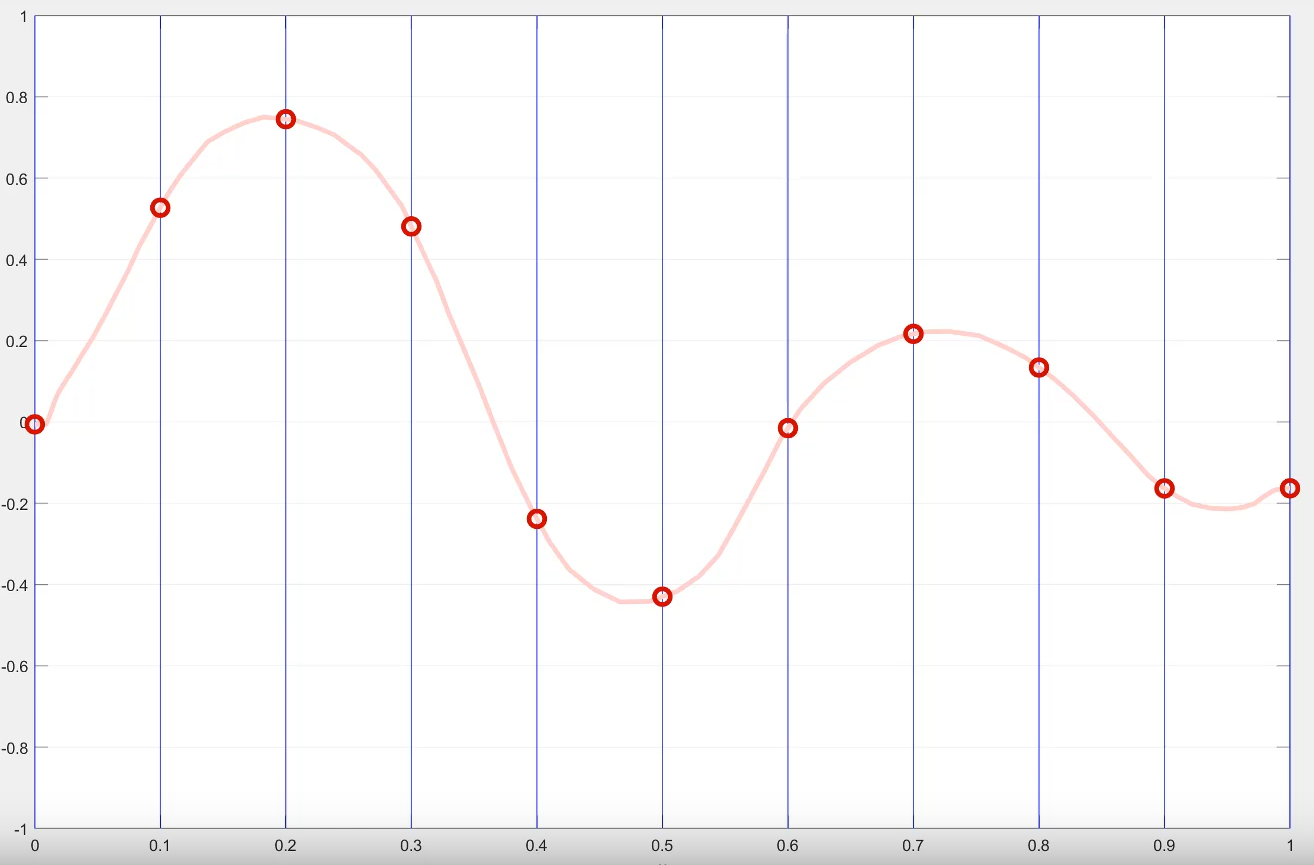
\includegraphics[width=0.99\linewidth]{figures/fdm.png}
      \caption{Finite difference}
      \label{fig:fdm}
    \end{subfigure}%
     \begin{subfigure}{.33\textwidth}
      \centering
      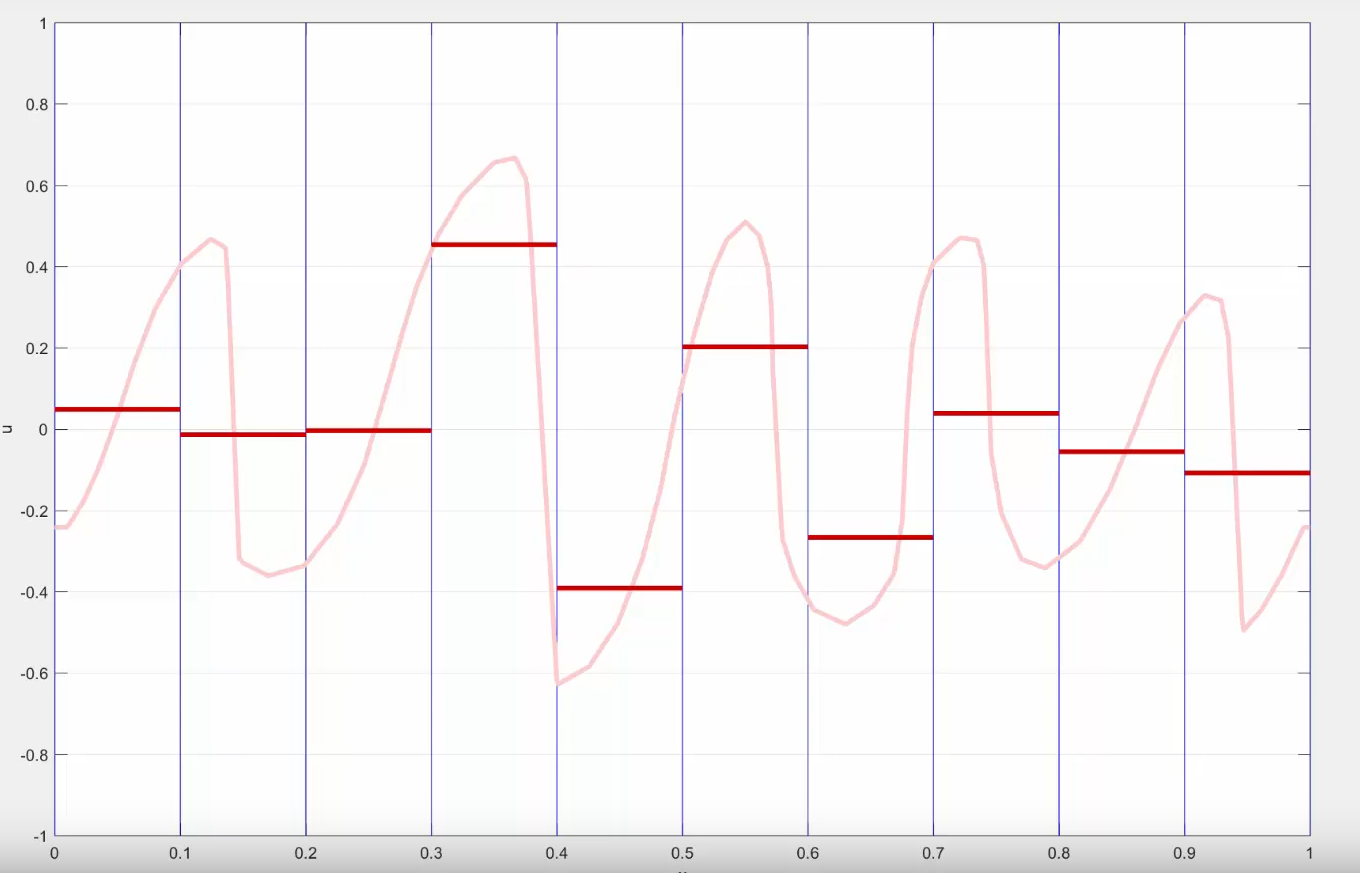
\includegraphics[width=.99\linewidth]{figures/fvm.png}
      \caption{Finite volume}
      \label{fig:fvm}
    \end{subfigure}%
	 	 \begin{subfigure}{.33\textwidth}
      \centering
      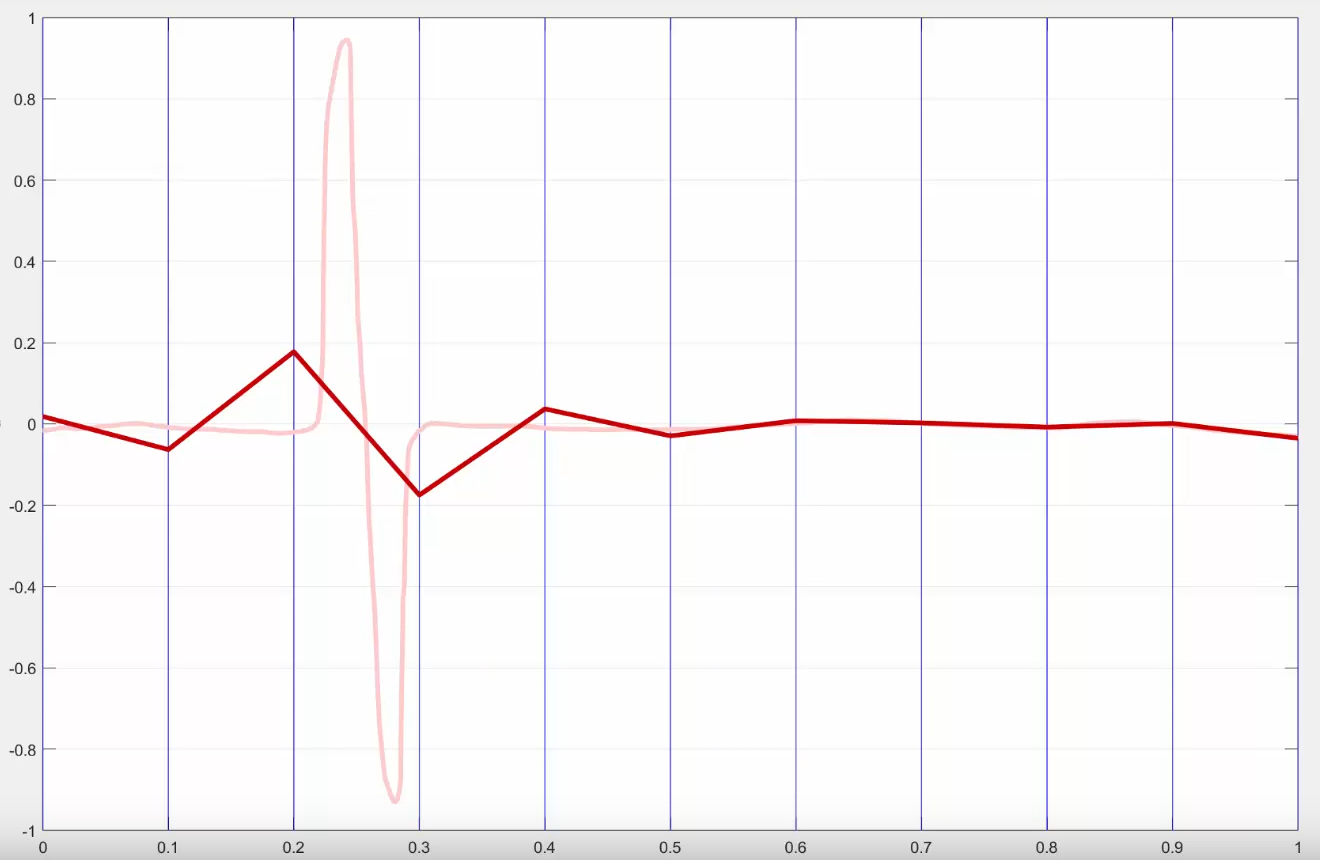
\includegraphics[width=.99\linewidth]{figures/fem.png}
      \caption{Finite element}
      \label{fig:fem}
    \end{subfigure}
	\caption{Comparison of numerical solution methods for partial differential equation: (a) finite difference (b) finite volume (c) finite element~\cite{pdesolution}.}
	\label{fig:pdesolution}
\end{figure}  

\subsection{Traditional Numerical Methods}
In numerical analysis, three common solution methods for PDEs exist: finite difference, finite volume and finite elements~\cite{pdesolution}. All of them approximate the arbitrary function using a finite number of discrete quantities. But the approximated quantities differ. The graphic comparison of these methods is shown in \cref{fig:pdesolution}.

\subsubsection{Finite Difference Method (FDM)} stores the values of the function of grid points. This is applied, when the computational costs have to be low.
\subsubsection{Finite Volumes Method (FVM)} stores the average values between the grid points. This is applied, when the conservation property is required e.g. energy equations. 
\subsubsection{Finite Element Methos (FEM)} chooses the best approximation within the finite dimension of possible basis functions (elements). FEM is the most flexible, but computational intensive compared to FDM and FVM.


%\subsection{Machine Learning Basics}